% =====================================================================
\section{Research gap and contributions}
\label{sec:gap}

The literature leads to four observations. (a) EEG and eye-tracking fusion consistently improves on single modalities \cite{Lu2015,Zheng2019,Liu2022}, but eye tracking is almost always used as a feature source rather than as an indicator of \emph{when} EEG carries affective information. (b) The only approach we found that uses eye tracking for temporal selection of EEG \cite{FarhadiSedehi2024a,FarhadiSedehi2024b} applies a crisp threshold to a single pupil feature. (c) The ocular signal used for gating is uncertain: it reflects arousal rather than a specific emotion, is confounded by luminance, cognitive load and gaze geometry, and contains missing and noisy samples \cite{Bradley2008,Mathot2018,Raiturkar2016,Holmqvist2012}. (d) Fuzzy soft weighting exists in related forms \cite{LinWang2002,Jacobs1991,Lu2015}, but our search found no study that maps eye-tracking memberships to continuous relevance weights for EEG windows.

Observations (b) and (c) are our analysis; the original authors acknowledge the limited input capacity of the S-FIS and the scarcity of multimodal databases \cite{FarhadiSedehi2024a}, not the brittleness of the threshold. A further gap is methodological: published evaluations of gating report only end-to-end accuracy on real data, where the relevance of each window is unknown, and use segment-level random cross-validation, in which windows from the same trial fall into both training and test sets \cite{FarhadiSedehi2024a,Li2021,Khan2025}. Neither allows the effect of the gate to be separated from other factors. This paper addresses that gap with a simulation in which relevance is known and with trial- and subject-disjoint evaluation. Combining EEG, eye tracking and fuzzy logic is not novel in itself \cite{Lu2015,FarhadiSedehi2024a}; the specific question studied is the \emph{form of the eye-tracking gate}, with all other components fixed. Our literature search was not a formal systematic review, so the novelty claim is stated to the best of our knowledge.

% =====================================================================
\section{Methodology}
\label{sec:method}

\subsection{Overall architecture}
Figure~\ref{fig:arch} shows the architecture shared by all compared configurations. The EEG branch (preprocessing, windowing, DWT band decomposition, entropy features, mRMR selection and S-FIS-GA classification) and the eye-tracking feature branch are identical; configurations differ only in the gate, which converts the gating feature of each window into a weight $w_k$. Table~\ref{tab:notation} lists the notation. The implementation follows the description in \cite{FarhadiSedehi2024a}; where that description is incomplete, the choice made is stated explicitly.

%ARCHFIG%

\begin{table}[t]
\centering\small
\caption{Key notations}\label{tab:notation}
\begin{tabular}{@{}ll@{}}
\toprule
Notation & Description\\
\midrule
$n$, $k$, $K_n$ & Trial index; window index; number of windows in trial $n$ ($K_n=15$)\\
$\mathbf{x}_{n,k}\in\mathbb{R}^{3}$ & Selected EEG entropy features of window $k$ (S-FIS inputs)\\
$z_{n,k}$, $\tilde z_{n,k}$ & Raw and normalised gating feature of window $k$\\
$\mu_{L},\mu_{M},\mu_{H}$ & Low/Medium/High membership functions of the fuzzy gate\\
$r_{L},r_{M},r_{H}$ & Constant consequents (relevance levels) of the gate rules\\
$w_{n,k}$ & Window weight: $\{0,1\}$ for M0, $[r_L,1]$ for M1\\
$\alpha_j(\mathbf{x})$, $\mathrm{CF}_j$ & Firing strength and certainty factor of classification rule $j$\\
$p_{n,k,c}$, $S_{n,c}$ & Window class score; aggregated trial score for class $c$\\
$C$ & Number of classes ($C=4$)\\
\bottomrule
\end{tabular}
\end{table}

\subsection{Shared EEG pipeline}
\paragraph{Preprocessing and windowing.} EEG is band-pass filtered (fourth-order zero-phase Butterworth, 1--60~Hz), notch-filtered at 50~Hz ($Q=30$) and resampled to 128~Hz, following \cite{FarhadiSedehi2024a}. Each 60-s trial is divided into $K_n=15$ non-overlapping 4-s windows.

\paragraph{Band decomposition.} A four-level DWT with the Daubechies-4 wavelet \cite{Mallat1989} yields, at 128~Hz, the sub-bands A4 (0--4~Hz, delta), D4 (4--8~Hz, theta), D3 (8--16~Hz, alpha), D2 (16--32~Hz, beta) and D1 (32--64~Hz, gamma). These dyadic boundaries only approximate the conventional bands quoted in \cite{FarhadiSedehi2024a}. Each sub-band is reconstructed to full length before windowing, so entropies are computed on 512-sample signals rather than on decimated coefficient vectors, which would be too short for embedding dimension 5.

\paragraph{Entropy features.} For each channel, sub-band and window, four entropies are computed with the parameters of \cite{FarhadiSedehi2024a}: sample entropy \cite{Richman2000}
\begin{equation}
\mathrm{SampEn}(m,r) = -\ln\frac{A}{B},
\end{equation}
where $B$ and $A$ count template pairs of length $m$ and $m+1$ within tolerance $r$ (self-matches excluded), with $m=5$, delay 2 and $r=0.15\,\sigma$; permutation entropy \cite{Bandt2002}
\begin{equation}
\mathrm{PermEn} = -\sum_{i=1}^{m!} p_i \ln p_i,
\end{equation}
with order $m=5$ and delay 2; symbolic dynamics entropy \cite{Zebrowski2000} with word length 5, delay 2 and alphabet size 3; and phase entropy \cite{Rohila2019}
\begin{equation}
\mathrm{PhEn} = -\sum_{i=1}^{k} p(i)\log p(i)
\end{equation}
over $k=5$ sectors of the second-order difference plot. With 62 channels, each window yields $4\times62=248$ features per band. Features are z-scored per subject, which uses no labels.

\paragraph{Weighted feature selection.} Three features per band are selected with the mRMR criterion \cite{Peng2005}
\begin{equation}
f_{t+1} = \arg\max_{f_j\notin\mathcal{S}_t}\Big[I_w(f_j;y) - \frac{1}{|\mathcal{S}_t|}\sum_{f_i\in\mathcal{S}_t} I_w(f_j;f_i)\Big],
\label{eq:mrmr}
\end{equation}
where $I_w$ is the mutual information of features discretised into 10 quantile bins, computed from a contingency table in which each training window contributes its weight $w_{n,k}$. For binary weights this is ordinary mRMR on the retained windows.

\paragraph{Sugeno fuzzy classifier.} Each selected feature is partitioned into three levels (Low, Medium, High) by greedy entropy-based discretisation of the (weighted) training data, and triangular membership functions with shoulders are centred on the resulting intervals \cite{FarhadiSedehi2024a}. Candidate rules
\begin{equation}
R_j:\ \text{IF } x_1 \text{ is } A_{j1} \text{ AND } x_2 \text{ is } A_{j2} \text{ AND } x_3 \text{ is } A_{j3} \text{ THEN class} = c_j \text{ with } \mathrm{CF}_j
\end{equation}
are generated by the look-up-table method \cite{WangMendel1992}: each training window proposes the antecedent formed by its maximum-membership levels with degree $w_{n,k}\prod_i\max_\ell\mu_{i\ell}(x_i)$, and conflicting rules keep the class with the largest summed degree. The firing strength uses the product t-norm, $\alpha_j(\mathbf{x})=\prod_{i}\mu_{A_{ji}}(x_i)$, and the window class score is the zero-order Sugeno output with class-indicator consequents,
\begin{equation}
p_{n,k,c} = \frac{\sum_{j:\,c_j=c}\mathrm{CF}_j\,\alpha_j(\mathbf{x}_{n,k})}{\sum_{j}\mathrm{CF}_j\,\alpha_j(\mathbf{x}_{n,k})},
\label{eq:score}
\end{equation}
with the class prior used when no rule fires.

\paragraph{GA rule tuning.} The GA encodes, for every mined rule, an activity bit and its antecedent levels (including ``don't care''); consequents and certainty factors are recomputed from the weighted training data for each candidate (class of maximum weighted firing mass; certainty factor equal to confidence minus the mean confidence of the other classes). The population size is 27 \cite{FarhadiSedehi2024a}, with two elite individuals, tournament selection of size 3, rule-level uniform crossover (rate 0.8), activity and antecedent mutation (rate 0.05 each) and termination after 10 generations without improvement (maximum 500). The fitness combines accuracy and coverage as in \cite{FarhadiSedehi2024a}, both weighted by the window weights, with a small rule-count penalty:
\begin{equation}
\Phi = \mathrm{Acc}_w + 0.2\,\mathrm{Cov}_w - 0.01\,\frac{R_{\mathrm{active}}}{R},\quad
\mathrm{Acc}_w = \frac{\sum w_{n,k}\mathbf{1}[\hat y_{n,k}=y_n]}{\sum w_{n,k}},\quad
\mathrm{Cov}_w = \frac{\sum w_{n,k}\mathbf{1}[\exists j:\alpha_j>0]}{\sum w_{n,k}}.
\label{eq:fit}
\end{equation}

\paragraph{Weighted trial-level aggregation.} Window scores are combined into a trial prediction with the same weights,
\begin{equation}
S_{n,c} = \frac{\sum_{k=1}^{K_n} w_{n,k}\,p_{n,k,c}}{\sum_{k=1}^{K_n} w_{n,k}},\qquad \hat y_n = \arg\max_{c} S_{n,c},
\label{eq:agg}
\end{equation}
which is a weighted sum rule \cite{Kittler1998}. Every configuration therefore produces exactly one prediction for every trial, so all are evaluated on the same set of trials.

\subsection{Eye-tracking features and gating feature}
Eight features are computed per 4-s window as in \cite{FarhadiSedehi2024a}: mean, standard deviation and maximum of fixation duration, fixation frequency, and mean and standard deviation of pupil diameter in the horizontal and vertical directions; blink samples are excluded. Two ways of choosing the gating feature are studied. In \textbf{G-pupil}, the gate uses the mean vertical pupil diameter, the feature reported by \cite{FarhadiSedehi2024a}. In \textbf{G-mRMR}, the original selection procedure is reproduced: the eight features are z-scored per subject, ranked by mRMR against the class label on the training windows of each fold, and the top-ranked feature is used.

The gating feature is normalised within each trial with robust percentile scaling, which uses no labels:
\begin{equation}
\tilde z_{n,k} = \operatorname{clip}_{[0,1]}\left(\frac{z_{n,k}-P_{5}^{(n)}}{P_{95}^{(n)}-P_{5}^{(n)}}\right),
\label{eq:norm}
\end{equation}
where $P_{5}^{(n)}$ and $P_{95}^{(n)}$ are percentiles over the windows of trial $n$.

\subsection{Hard gate (M0)}
The original description uses ``the maximum'' of the gating feature as threshold without specifying its scope or how many windows are kept. Read literally, it would keep a single window per trial. Following the team's implementation, the threshold is the within-trial 60th percentile,
\begin{equation}
w^{\mathrm{M0}}_{n,k} = \mathbf{1}\big[\tilde z_{n,k} \geq Q_{0.6}^{(n)}(\tilde z)\big],
\label{eq:hard}
\end{equation}
which retains about 40\% of the windows of every trial; windows with $w=0$ are excluded from all training steps and from aggregation.

\subsection{Fuzzy gate (M1)}
\paragraph{Fuzzification.} The normalised feature is described by three fuzzy sets forming a Ruspini partition ($\mu_L+\mu_M+\mu_H=1$):
\begin{align}
\mu_{L}(\tilde z) &= \operatorname{clip}_{[0,1]}\!\Big(\frac{c-\tilde z}{c-a_1}\Big),\qquad
\mu_{H}(\tilde z) = \operatorname{clip}_{[0,1]}\!\Big(\frac{\tilde z-c}{b_2-c}\Big),\\
\mu_{M}(\tilde z) &= \max\!\Big(0,\min\!\Big(\frac{\tilde z-a_1}{c-a_1},\frac{b_2-\tilde z}{b_2-c}\Big)\Big),
\end{align}
with $a_1=0.2$, $c=0.5$ and $b_2=0.8$ (Fig.~\ref{fig:mf}a). These values were fixed a priori and not tuned.

\paragraph{Gate rule base and weight.} A zero-order Sugeno rule base maps memberships to relevance: IF $\tilde z$ is Low THEN relevance $=r_L$; IF $\tilde z$ is Medium THEN relevance $=r_M$; IF $\tilde z$ is High THEN relevance $=r_H$, with $(r_L,r_M,r_H)=(0.1,0.5,1)$. The weight is
\begin{equation}
w^{\mathrm{M1}}_{n,k} = \frac{\mu_L(\tilde z_{n,k})\,r_L + \mu_M(\tilde z_{n,k})\,r_M + \mu_H(\tilde z_{n,k})\,r_H}{\mu_L(\tilde z_{n,k})+\mu_M(\tilde z_{n,k})+\mu_H(\tilde z_{n,k})}\ \in [r_L,1],
\label{eq:fuzzy}
\end{equation}
so no window is discarded. If the Medium set shrinks to zero width at the threshold and $r_L\to0$, Eq.~\eqref{eq:fuzzy} reduces to a crisp step, so M0 is a limiting case of M1. With one input and a Ruspini partition, Eq.~\eqref{eq:fuzzy} is a monotone piecewise-linear function of $\tilde z$ (Fig.~\ref{fig:mf}b). To test whether the fuzzy formulation adds anything beyond softness, the linear soft gate $w^{\mathrm{A4}}_{n,k}=\max(r_L,\tilde z_{n,k})$ is included as an ablation.

\begin{figure}[t]
\centering
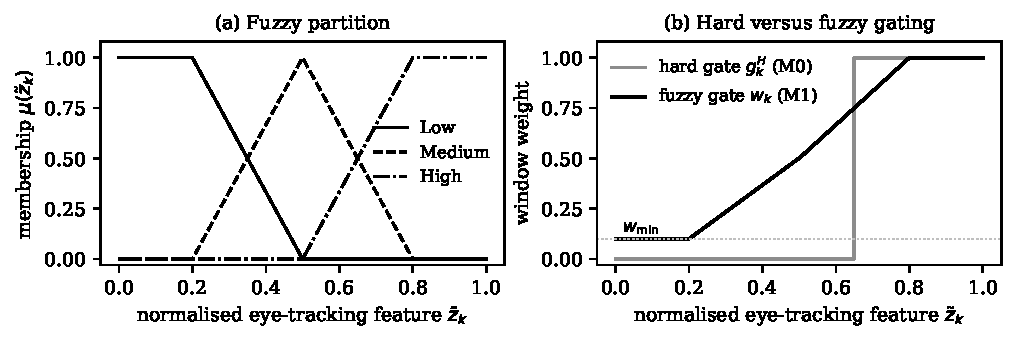
\includegraphics[width=0.95\linewidth]{figures/fuzzy_gate_mf.pdf}
\caption{(a) Fuzzy partition of the normalised gating feature. (b) Fuzzy gate weight (Eq.~\ref{eq:fuzzy}) compared with a hard gate. Parameters $a_1=0.2$, $c=0.5$, $b_2=0.8$, $r=(0.1,0.5,1)$; the hard-gate step is drawn at $\tau=0.65$ for illustration, whereas M0 places its threshold at the within-trial 60th percentile.}
\label{fig:mf}
\end{figure}

Algorithm~\ref{alg:m1} summarises one cross-validation fold, and Table~\ref{tab:m0m1} lists the components of every configuration.

\begin{algorithm}[t]
\caption{Gated S-FIS-GA recognition for one cross-validation fold}\label{alg:m1}
\small
\begin{algorithmic}[1]
\Require Training trials $\mathcal{T}$, test trials $\mathcal{V}$ (disjoint), gate type $\in\{$none, hard, fuzzy, linear$\}$
\Ensure Trial predictions $\{\hat y_n\}_{n\in\mathcal{V}}$
\State Compute 8 ET features and $5\times4\times62$ EEG entropies for every 4-s window
\State Choose gating feature (fixed pupil-Y, or mRMR rank on windows of $\mathcal{T}$)
\State Normalise it within each trial (Eq.~\ref{eq:norm}); compute $w_{n,k}$ (Eq.~\ref{eq:hard} or \ref{eq:fuzzy})
\For{each band}
  \State Select 3 EEG features by weighted mRMR on $\mathcal{T}$ (Eq.~\ref{eq:mrmr})
  \State Fit weighted entropy cut points and triangular MFs on $\mathcal{T}$
  \State Mine look-up-table rules with degrees scaled by $w_{n,k}$
  \State Tune the rule base with the GA using fitness $\Phi$ (Eq.~\ref{eq:fit})
  \For{each $n\in\mathcal{V}$} compute $p_{n,k,c}$ (Eq.~\ref{eq:score}) and $\hat y_n$ (Eq.~\ref{eq:agg}) \EndFor
\EndFor
\end{algorithmic}
\end{algorithm}

\begin{table}[t]
\centering\small
\caption{Components of the compared configurations; only the gate differs}\label{tab:m0m1}
\begin{tabular}{@{}lllll@{}}
\toprule
Component & A1 (no gate) & M0 (hard) & M1 (fuzzy) & A4 (linear)\\
\midrule
EEG pipeline, ET features & \multicolumn{4}{c}{shared (Sect.~4.2--4.3)}\\
Gating feature & -- & \multicolumn{3}{c}{G-pupil or G-mRMR (shared)}\\
Window weight & $1$ & Eq.~\eqref{eq:hard} & Eq.~\eqref{eq:fuzzy} & $\max(0.1,\tilde z)$\\
Effective share of training windows\simnote & 100\% & 41.8\% & 45.7\% & 44.3\%\\
Weights in mRMR, cuts, rule mining, GA & -- & \multicolumn{3}{c}{yes (Eqs.~\ref{eq:mrmr}, \ref{eq:fit})}\\
Trial aggregation & \multicolumn{4}{c}{Eq.~\eqref{eq:agg}}\\
\bottomrule
\end{tabular}
\end{table}

